\begin{frame}[t]{A Conjectura Jacobiana}
\small
\begin{teobox}{Conjectura Jacobiana (Keller, 1939)}
Seja $\KK$ algebricamente fechado e $F\colon\KK^n\to\KK^n$ polinomial.
Se $\det(J_F) \in \KK^*$ , então $F$ é automorfismo polinomial.
\end{teobox}
\vspace{0.5cm}
\begin{center}
    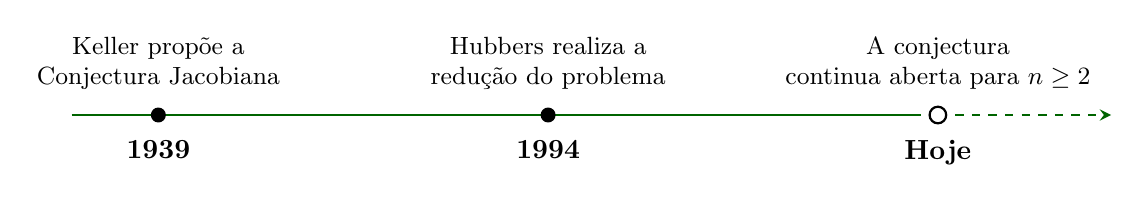
\begin{tikzpicture}[x=1.1cm, y=1cm, >=stealth]
        


        

        \draw[ thick, DarkGreen] (-1,0) -- (8.8,0);
        

        \draw[thick, dashed, DarkGreen, ->] (9.2,0) -- (11,0);

        \filldraw (0,0) circle (2.5pt);
        \node[below=0.2cm, font=\bfseries] at (0,0) {1939};
        \node[above=0.2cm, align=center, font=\small] at (0,0) {Keller propõe a\\Conjectura Jacobiana};
    

        \filldraw (4.5,0) circle (2.5pt);
        \node[below=0.2cm, font=\bfseries] at (4.5,0) {1994};
        \node[above=0.2cm, align=center, font=\small] at (4.5,0) {Hubbers realiza a\\redução do problema};
    

        \filldraw[fill=white, draw=black, thick] (9,0) circle (3pt);
        \node[below=0.2cm, font=\bfseries] at (9,0) {Hoje};
        \node[above=0.2cm, align=center, font=\small] at (9,0) {A conjectura\\continua aberta para $n \geq 2$};
        
    \end{tikzpicture}
\end{center}
\end{frame}